% Figure: scale covariance (A8) as a commuting square, with the scale axis relabelled.
% Referenced from §2.3. Pure TikZ, no external file. Design after the hub's
% scripts/covariance_square.py (SSF), adapted: the transported parameter is a *pair* of
% scales, and the relabelling S_σ is what (A8) leaves free.
%
% Pedagogic point: dilating the signal and then measuring equals measuring and then
% dilating — but at the transported scales (S_σ x, S_σ y). The lower strip shows the
% scale axis being carried onto itself by S_σ, which is why (A8) is stated with the
% relabelling left free and why the scale labels have no metric meaning until §6.

\begin{figure}[t]
\centering
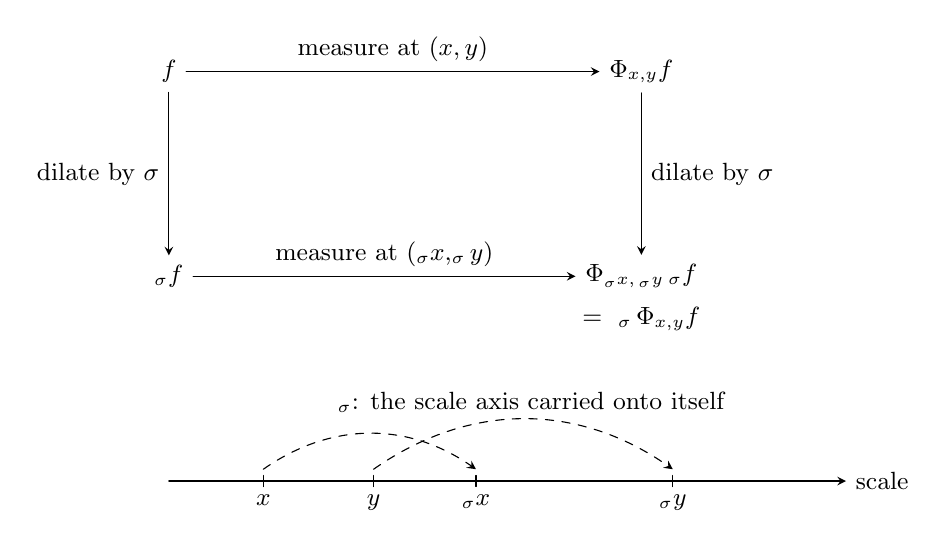
\begin{tikzpicture}[every node/.style={font=\small}, line cap=round, >=stealth]

% ---------- the commuting square ----------
\node (f)   at (0,2.6)   {$f$};
\node (Pf)  at (6.0,2.6) {$\Phi_{x,y} f$};
\node (Df)  at (0,0)     {$\dil_\sigma f$};
\node (PDf) at (6.0,0)   {$\Phi_{\Sact_\sigma x,\,\Sact_\sigma y}\,\dil_\sigma f$};
\node[anchor=north] at (PDf.south) {$=\ \dil_\sigma\,\Phi_{x,y} f$};

\draw[->] (f)  -- node[above] {measure at $(x,y)$} (Pf);
\draw[->] (f)  -- node[left]  {dilate by $\sigma$} (Df);
\draw[->] (Pf) -- node[right] {dilate by $\sigma$} (PDf);
\draw[->] (Df) -- node[above] {measure at $(\Sact_\sigma x, \Sact_\sigma y)$} (PDf);

% ---------- the scale axis, relabelled ----------
\begin{scope}[yshift=-2.6cm]
  \draw[->] (0,0) -- (8.6,0) node[right] {scale};
  \foreach \p/\l in {1.2/$x$, 2.6/$y$} {
    \draw (\p,0.07) -- (\p,-0.07); \node[below] at (\p,-0.05) {\l};
  }
  \foreach \p/\l in {3.9/$\Sact_\sigma x$, 6.4/$\Sact_\sigma y$} {
    \draw (\p,0.07) -- (\p,-0.07); \node[below] at (\p,-0.05) {\l};
  }
  \draw[->,dashed] (1.2,0.15) to[bend left=35] (3.9,0.15);
  \draw[->,dashed] (2.6,0.15) to[bend left=35] (6.4,0.15);
  \node[anchor=south] at (4.6,0.75) {$\Sact_\sigma$: the scale axis carried onto itself};
\end{scope}

\end{tikzpicture}
\caption{Scale covariance (A8). Dilating the signal by $\sigma$ and then measuring is
the same as measuring and then dilating, provided the measurement is taken at the
transported scales $(\Sact_\sigma x, \Sact_\sigma y)$: the square commutes. The lower
strip shows the relabelling. Nothing ties the scale labels to a unit of time at this
stage, so (A8) can only ask that the family be mapped onto itself, with the labels
rearranged by some increasing bijection $\Sact_\sigma$; \S\ref{sec:covariance} shows
that the axioms determine $\Sact_\sigma$ and thereby a canonical parametrization of the
scale axis.}
\label{fig:covariance-square}
\end{figure}
